\documentclass{article}
\usepackage{iclr2016_conference,times}

\usepackage{float}
\usepackage{hyperref}
\usepackage{url}
\usepackage{amsmath,amssymb}
\usepackage{natbib}
\usepackage{wrapfig}
\usepackage{graphicx}
\usepackage{subfig}

\bibliographystyle{abbrvnat}


\usepackage{caption}
%\usepackage{subcaption}

\title{
	Mobile Computing (CS23400$/$1) \vspace{-4pt} \\
	{\Large Lab 2 - Report} \vspace{6pt} \\
	{\large Andrea F. Daniele $\hspace{2.2cm}$ Max X. Liu $\hspace{2.2cm}$ Noah A. Hirsch}
}

\begin{document}

\maketitle


\vspace{-1.2cm}

\section{Task and Challenges}
\vspace{-.3cm}
\begin{wrapfigure}{r}{0.4\textwidth}
    \centering
    \vspace{-14pt}
    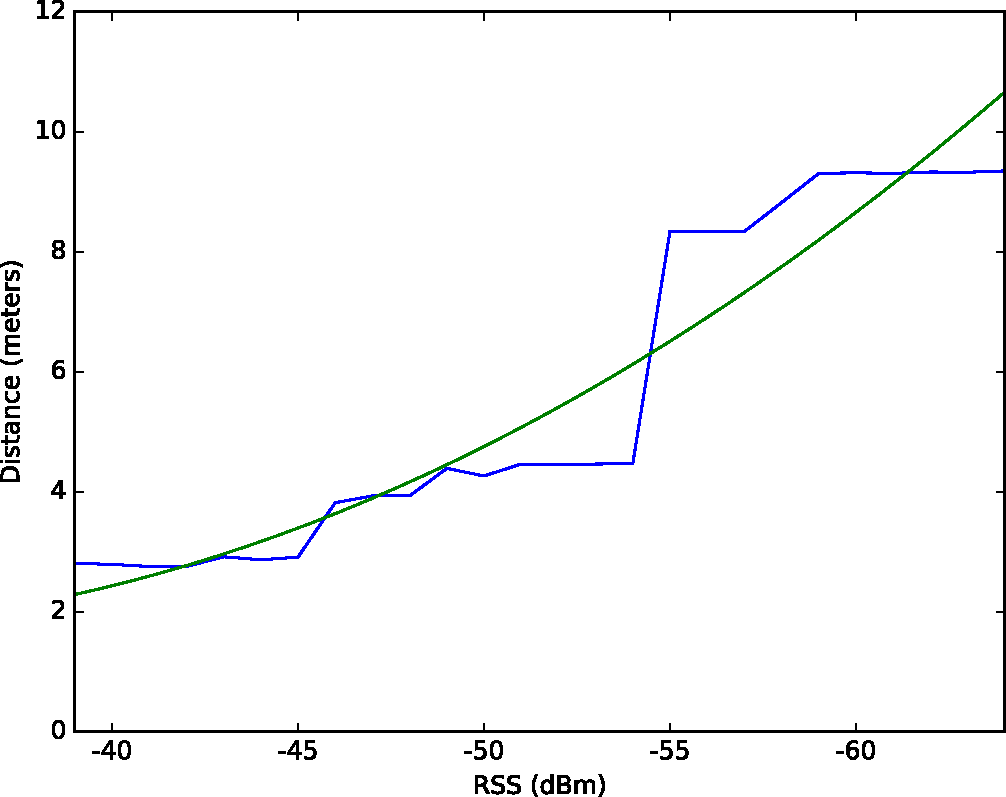
\includegraphics[width=\linewidth]{figures/rss_distance_plot.pdf}
    \caption{RSS-Distance relationship \label{fig:rss_distance_plot}}
    \vspace{-28pt}
\end{wrapfigure}
The goal of this lab is to identify the location of a Wi-Fi device by analyzing Received Signal Strength 
(RSS) data recorded by a Wi-Fi receiver mounted on a moving car. The main challenge in this lab is
mitigating RSS noise. Another challenge is that while collecting data, our car would often turn on its 
own, which would make it difficult to determine the car's position from its starting point, stopping point, 
and speed. We don't address this last limitation in this lab.


\section{Proposed Approach}
\vspace{-.3cm}
\begin{wrapfigure}{r}{0.4\textwidth}
    \centering
    \vspace{-20pt}
    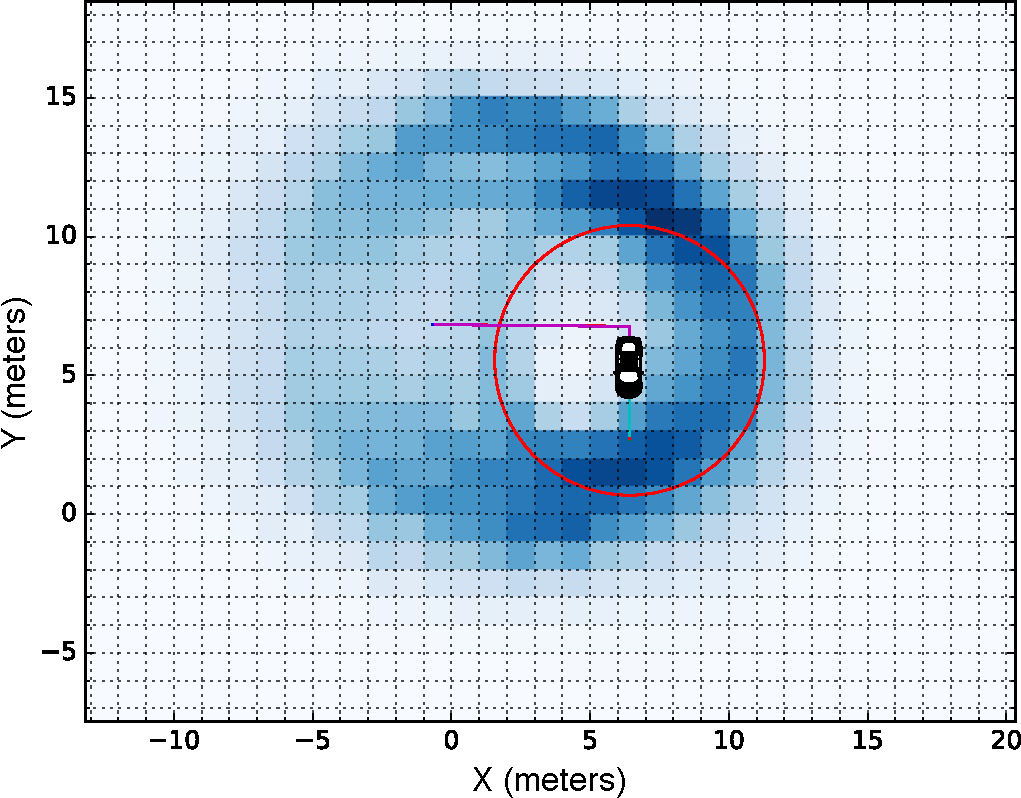
\includegraphics[width=\linewidth]{figures/moving_car.pdf}
    \caption{Heat map resulting from the intersection of multiple RSS readings \label{fig:moving_car}}
    \vspace{-20pt}
\end{wrapfigure}
For each RSS reading, we estimate the distance from the car to the Wi-Fi device and thus create a 
circular locus of possible locations around the car. The relationship between RSS and distance
from the transmitter is modeled using a second order polynomial function. We fit this function to the 
data for which the distance from the transmitter is known (shown in Fig.~\ref{fig:rss_distance_plot}).

As we collect multiple RSS readings from the moving car, we can create multiple loci whose 
intersection locates the position of the Wi-Fi device.
Fig.~\ref{fig:moving_car} shows how we intersect multiple RSS readings relative to the same device
on a 2D discretized representation of the environment. The blue heat-map shows the current 
probability distribution over locations for a specific WiFi device. The red circle has its center on the
car's position and radius corresponding to the estimated distance based on the current RSS reading. 
It is worth noting that the center of the darkest cell in the heat-map of Fig.~\ref{fig:moving_car}
(cell with highest probability) has coordinates $(7.5, 10.5)$, which corresponds to the location 
predicted by our model for the device 8c:85:90:16:0a:a4 (shown later in Table~\ref{tab:results}).

We must also overcome the RSS noise 
due to variable environments and signal reflection.
To resolve this, our method chooses the single location in the workspace with the most locus 
intersections. 
\begin{wrapfigure}{r}{0.4\textwidth}
    \centering
    \vspace{-4pt}
    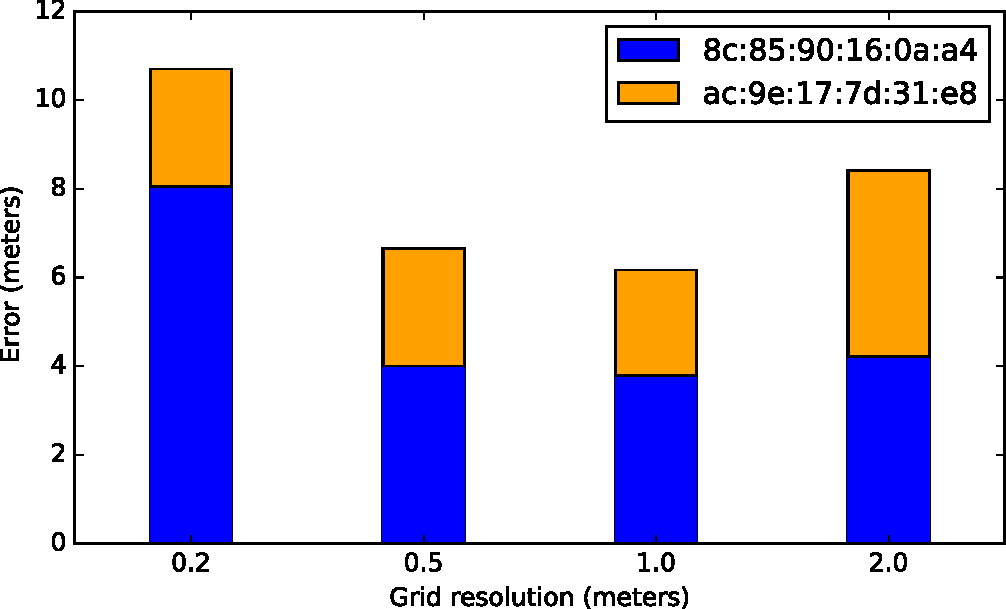
\includegraphics[width=\linewidth]{figures/grid_resolution_study.pdf}
    \caption{Localization error for the devices with known location \label{fig:grid_resolution_study}}
    \vspace{-10pt}
\end{wrapfigure}
Since we are collecting hundreds of RSS datapoints each second, the truthful 
datapoints will converge on the correct location, while the noisy datapoints will not converge on 
a single location as much to outweigh that correct answer. We believe this to be an appropriate 
solution, and it will be shown later that it can detect the location of two test Wi-Fi devices of 
which we know the location with a relatively small error.

We discretized the environment using a grid with resolution of $1.0$ meter. We based this decision 
on results from empirical experiments run on the two WiFi devices for which the ground-truth location 
is known. Fig.~\ref{fig:grid_resolution_study} shows the localization error for the both devices and 
for four different grid resolutions.



\begin{figure}[t]
    \centering
    \subfloat[Device with MAC d8:c4:6a:50:e3:b1]{{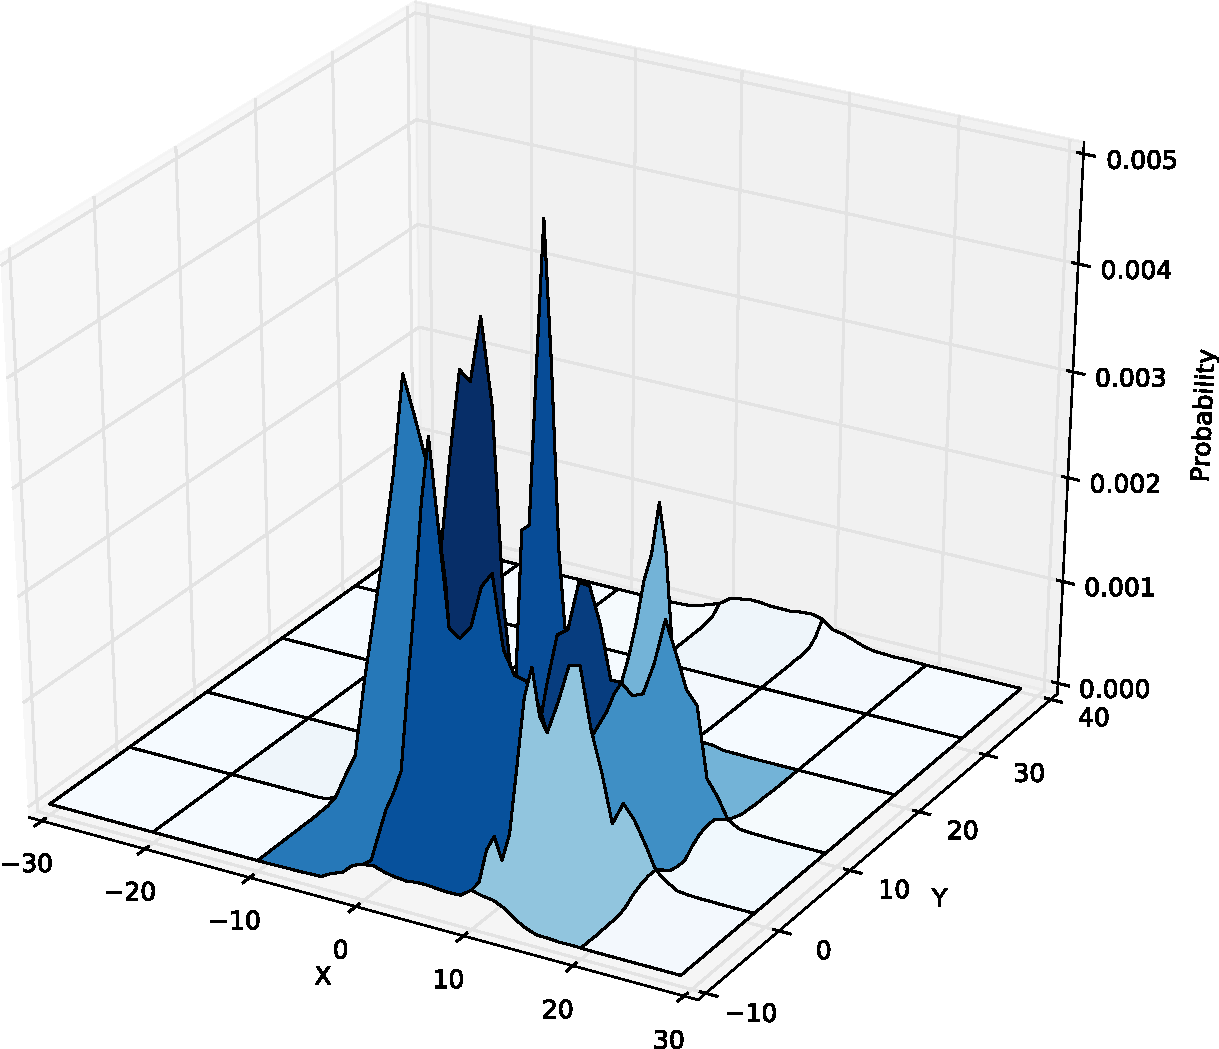
\includegraphics[width=0.46\linewidth]{figures/pdist_d8_b1.pdf} }}%
    \qquad
    \subfloat[Device with MAC f8:cf:c5:97:e0:9e]{{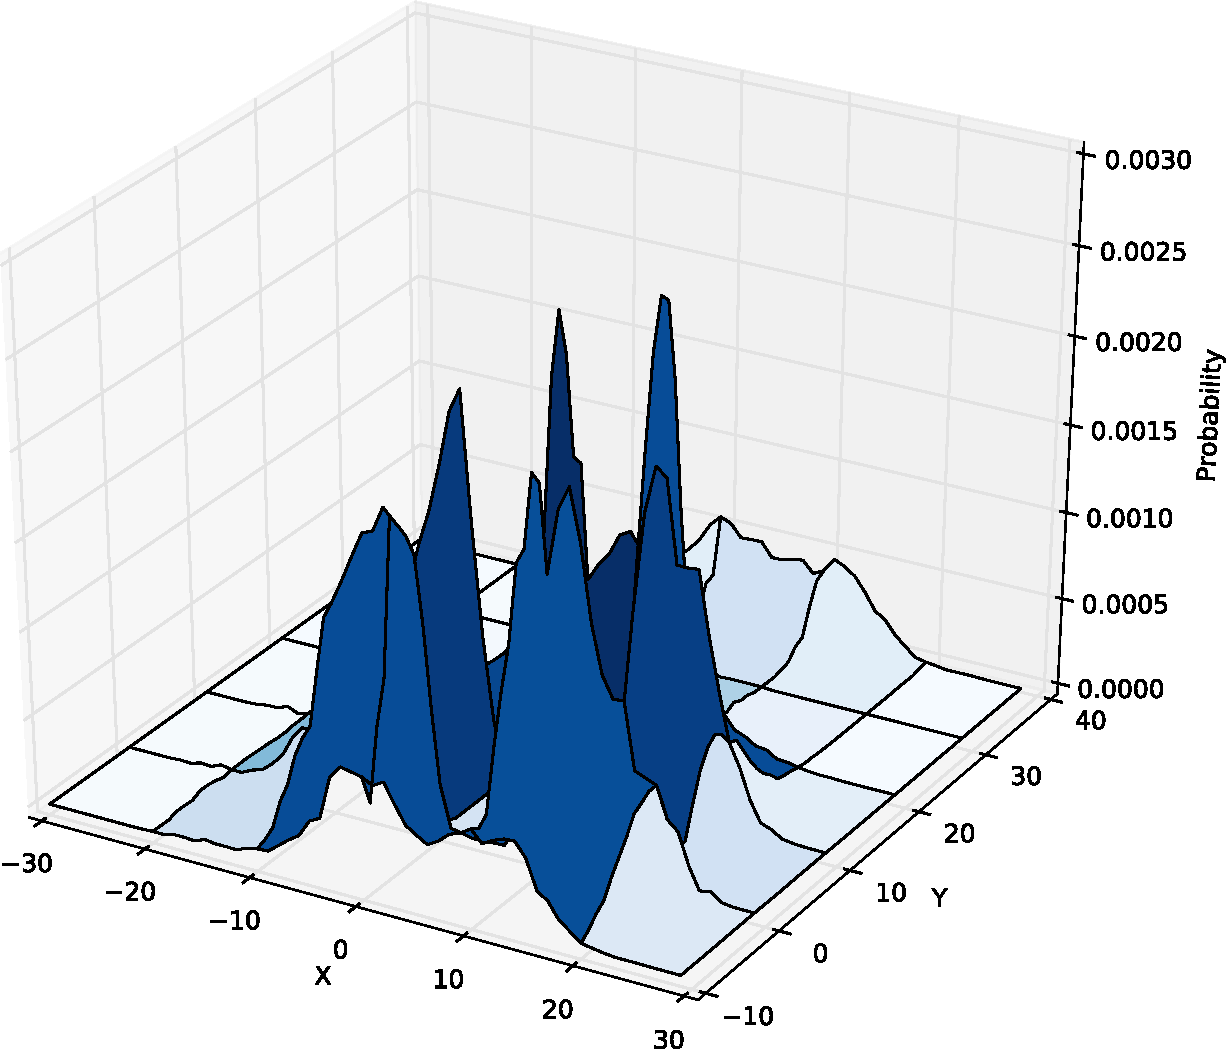
\includegraphics[width=0.46\linewidth]{figures/pdist_f8_9e.pdf} }}%
    \caption{Probability distributions over locations for the two devices with unknown locations}%
    \label{fig:pdists_hidden_cameras}%
\end{figure}

\section{Results}
\vspace{-.3cm}
We tested our approach on two WiFi camera for which we know the true location. Our
model predicted the location of the two cameras with $3.77$ and $2.37$ meters error.
Table~\ref{tab:results} shows the predicted location along with the prediction error for the
cameras for which the true location is known and the predicted locations for the hidden cameras.
Fig.~\ref{fig:pdists_hidden_cameras} shows the final probability distributions over locations for the
devices for which the ground-truth location is unknown.

\begin{table}[h]
\centering
\begin{tabular}{ |c|c|c|c| } 
 \hline
 MAC & Predicted location (meters) & True location (meters) & Error (meters) \\ 
 \hline
 8c:85:90:16:0a:a4 & $(7.5, 10.5)$ & $(6.8, 6.8)$ & $3.77$\\ 
 ac:9e:17:7d:31:e8 & $(1.5, 9.5)$ & $(0.87, 9.45)$ & $2.37$ \\ 
 d8:c4:6a:50:e3:b1 & $(0.5, 14.5)$ & $-$ & $-$ \\
 f8:cf:c5:97:e0:9e & $(9.5, 16.5)$ & $-$ & $-$ \\
 \hline
\end{tabular}
 \caption{Predicted location and prediction error for four distinct WiFi devices \label{tab:results}}
\end{table}


\section{Conclusion}
\vspace{-.3cm}
Our approach proved to be able to estimate the location of a WiFi device simply based on
noisy observations of the RSS indicator with an average accuracy of $3.07$ meters.
During our experiments, we noticed that our approach produce better estimations when 
a high number of readings is available. In particular, Fig.~\ref{fig:grid_resolution_study} shows
that regardless of the grid resolution we choose, 
the estimation error is always smaller for the device with MAC address ac:9e:17:7d:31:e8
for which we have about $171k$ readings, compared to the device with MAC address
8c:85:90:16:0a:a4 for which we have only $43k$ readings.

\bibliographystyle{abbrvnat}
{\scriptsize%
\bibliography{references}
}

\end{document}
